\section{Controller in time domain}

% State feedback controller
\subsection{State feedback controller}
In a first time, we need to compute the gain matrix $K$.\par
In order not to apply a gain on the wind force, the matrix K is as follows :
$$
K = \begin{pmatrix}
    0 & 0 & 0 & 0\\ 
    g_1 & g_2 & g_3 & g_4
\end{pmatrix}
$$
Indeed, the first column of matrix B concerns the uncontrollable input, so matrix K cannot affect these values.\par
The new dynamic matrix of the closed-loop system is $A_{CL} = A - BK$. Let's determine the eigenvalues of that matrix.\par
As we have a matrix of dimension $4$, the approximation of the dominant poles will be done. Indeed, we have, from the previous matrix $A$, the eigenvalues :
\begin{align*}
    \lambda_1 &= \num{-0.0634 + 6.2837i}\\
    \lambda_2 &= \num{-0.0634 - 6.2837i}\\
    \lambda_3 &= \num{-0.1666 + 1.8179i}\\
    \lambda_4 &= \num{-0.1666 - 1.8179i}
\end{align*}
As already discussed in section \ref{sec:eigenvalues}, one can see that $\lambda_3$ and $\lambda_4$ are about 10 times bigger than the last two. They are not dominant when affecting the dynamics of the system, and will therefore remain in $A_{CL}$, although slightly modified, as explained after.\par
Imposing that $(s - \lambda_3)(s - \lambda_4)$ is part of the decomposition, we get that the determinant of $A_{CL}$ is equal to :
$$
(s - \lambda_3)(s - \lambda_4)(s^2 + 2 \zeta\omega_c s + \omega_c^2) = 0
$$
Since $\lambda_3$ and $\lambda_4$ are fixed, we only need to solve the equation of the second degree in $s$ in order to find the expressions of $\lambda_1'$ and $\lambda_2'$ as a function of $\zeta$ and $\omega_c$.\par
The solutions of the equation are given by :
$$
\begin{cases}
    \lambda_1' = -\zeta\omega_c - \omega_c\sqrt{\zeta^2 - 1}\\
    \lambda_2' = -\zeta\omega_c + \omega_c\sqrt{\zeta^2 - 1}
\end{cases}
$$
The values of $\zeta$ and $\omega_c$ will be determined by simulations in the following sections. When these have been fixed, the values of the 4 poles of $A_{CL}$ will be obtained. Then we will just have to use the \texttt{place} function of Matlab to obtain the values $g_i$ of matrix $K$ associated with the eigenvalues.\par
However, as previously noted via simulations, our system is very reactive. The two non-dominant eigenvalues thus have also been modified in order to slow down the system. We finally obtain the expressions of the 4 eigenvalues of the controller :
$$
\begin{cases}
    \lambda_1' = -\zeta\omega_c - \omega_c\sqrt{\zeta^2 - 1}\\
    \lambda_2' = -\zeta\omega_c + \omega_c\sqrt{\zeta^2 - 1}\\
    \lambda_3' = \mathbb{R}(\lambda_3)0.5 + \mathbb{I}(\lambda_3)i\\
    \lambda_4' = \mathbb{R}(\lambda_4)0.5 + \mathbb{I}(\lambda_4)i
\end{cases}
$$
As the reference is 0, $k_r$ has not to be considered, so it can fixed to 0.\par
However, some tests of a change in reference will be performed in this report. We therefore calculated $k_r$ using the following formula :
$$
k_r = \frac{-1}{C(A - BK)^{-1} B}
$$
where only the controllable part of matrix B (second column) and the non-zero row of K were considered. Indeed, if the entire matrices were used, it would mean that we would have an action on the uncontrollable input, which is not possible.

% Observer
\subsection{Observer}
The controllable input being a linear combination of the different states multiplied by gains, the control system requires the different states as inputs. However, the open loop system only provides one output.\par
Considering that the real states cannot be measured in practice, the observer is a tool that allows us, based only on the output of the open loop system and on the inputs, to approximate the different states of the system.\par
Its realization must be such that the convergence of the estimated states with the real states is as fast and correct as possible.\par
One thus needs to compute the gain matrix $L$ :
$$
L = \begin{pmatrix}
    l_1\\
    l_2\\
    l_3\\
    l_4
\end{pmatrix}
$$
The new dynamic matrix is given by $A_{obs} = A - LC$.\par
As previously, we will keep the same two non-dominant eigenvalues and determine the two other via the same method that has been used for $K$.\par
Imposing that $(s - \lambda_3')(s - \lambda_4')$ is part of the decomposition, we get that the determinant of $A_{obs}$ is equal to :
$$
(s - \lambda_3')(s - \lambda_4')(s^2 + 2 \zeta\omega_c s + \omega_c^2) = 0
$$
Since $\lambda_3'$ and $\lambda_4'$ are fixed, we only need to solve the equation of the second degree in $s$ in order to find the expressions of $\lambda_1^*$ and $\lambda_2^*$ as a function of $\zeta$ and $\omega_c$.\par
The solutions of the equation are given by :
$$
\begin{cases}
    \lambda_1^* = -\zeta\omega_c - \omega_c\sqrt{\zeta^2 - 1}\\
    \lambda_2^* = -\zeta\omega_c + \omega_c\sqrt{\zeta^2 - 1}
\end{cases}
$$
The poles of the observer are determined by taking the poles of the controller and moving them. To do this, the real parts of each pole are multiplied by a constant $\alpha$. In the case of poles $\lambda_1'$ and $\lambda_2'$, this amounts to multiplying $\omega_c$ by $\alpha$.\par
We finally have :
$$
\begin{cases}
    \lambda_1^* = -\zeta\omega_c\alpha - \omega_c\alpha\sqrt{\zeta^2 - 1}\\
    \lambda_2^* = -\zeta\omega_c\alpha + \omega_c\alpha\sqrt{\zeta^2 - 1}\\
    \lambda_3^* = \mathbb{R}(\lambda_3')\alpha + \mathbb{I}(\lambda_3')i\\
    \lambda_4^* = \mathbb{R}(\lambda_4')\alpha + \mathbb{I}(\lambda_4')i
\end{cases}
$$
The values $l_i$ of the matrix $L$ are then obtained by using the \texttt{place} function of Matlab. The chosen values are given in the next section.

% Simulations and discussion
\subsection{Simulations and discussion}
\subsubsection{Parameter determination}
In order to best achieve our control system, we must determine the values of $\zeta$, and $\omega_c$. We know that the system control is done via the controllable input $u(t)$, and that this input will influence the variation of the output and the different states of the system.\par
In order to obtain a coherent system, {\it i.e.} physically possible state values and an attenuation of building oscillations, we must choose values of $\zeta$ and $\omega_c$ that will lead to a control input making the system coherent.\par
We tested several values of $\zeta$ as well as several values of $\omega_c$ with a constant wind force~:
\begin{figure}[H]
    \centering
    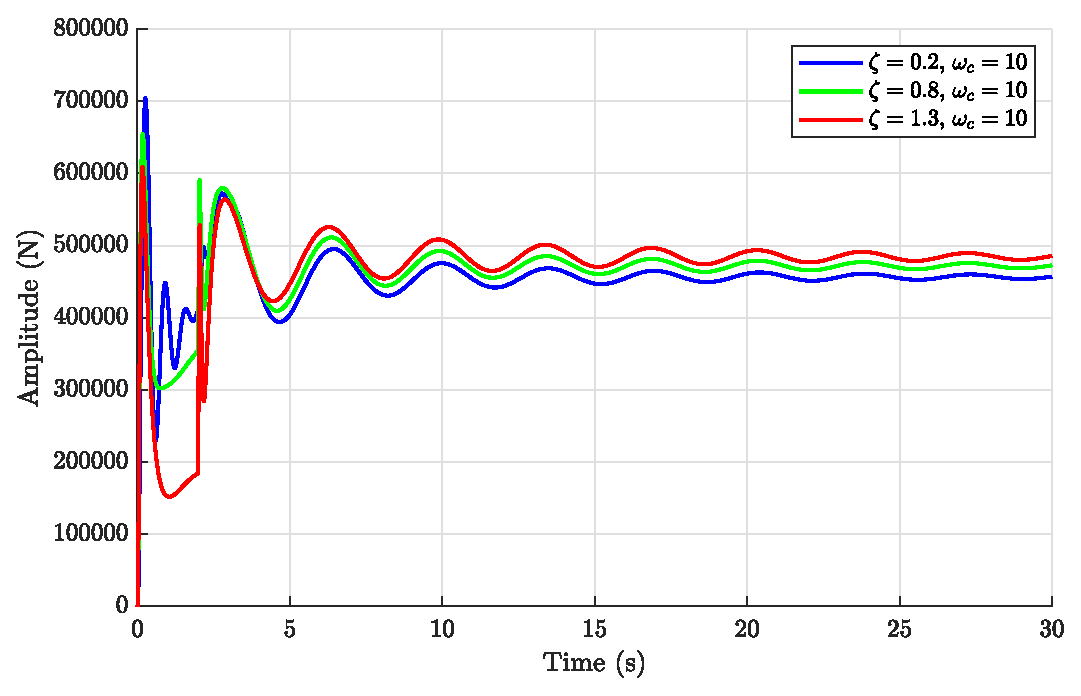
\includegraphics[width=\textwidth]{resources/eps/3_zeta-variations.eps}
    \caption{Control input $u(t)$ for different variations of parameter $\zeta$}
\end{figure}
\begin{figure}[H]
    \centering
    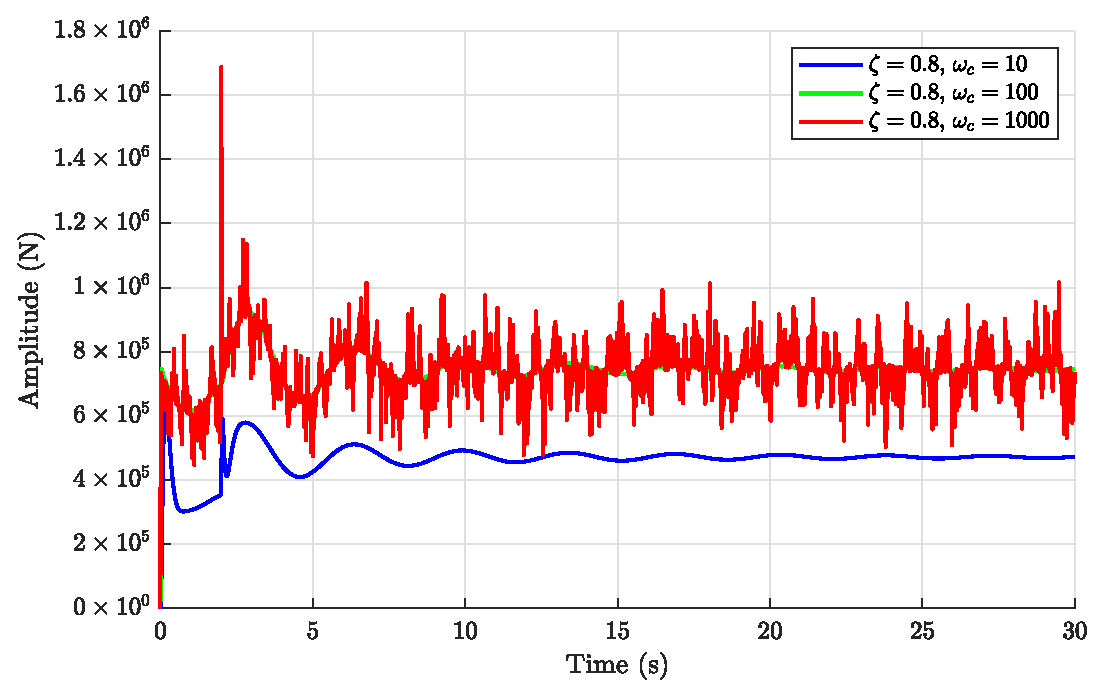
\includegraphics[width=\textwidth]{resources/eps/3_omega-variations.eps}
    \caption{Control input $u(t)$ for different variations of parameter $\omega_c$}
\end{figure}
It can be seen that the variations in parameter $\zeta$ have little influence on the controllable force : after a few seconds, it is identical in all cases.\par
Concerning the parameter $\omega_c$, we observe that the higher it is, the faster the control force oscillates (which is an undesirable behaviour).\par
We also observed the variation of the parameter $\omega_c$ on the states $x_1$ (also the output) and $x_3$ of our system :
\begin{figure}[H]
    \centering
    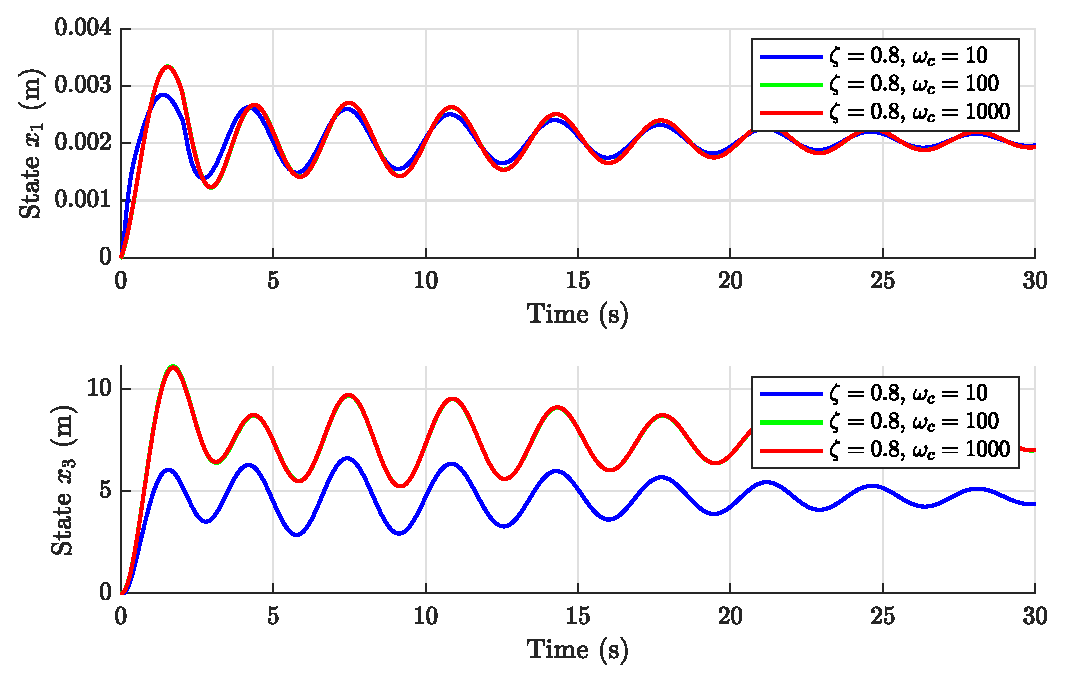
\includegraphics[width=\textwidth]{resources/eps/3_states-variations.eps}
    \caption{States $x_1$ and $x_3$ of the system for different variations of parameter $\omega_c$}
\end{figure}
First of all, we observe that the green and red curves overlap perfectly. Then, we find that the influence of the $\omega_c$ parameter on the states is relatively small. Only the damper's behaviour varies considerably.\par
The variations of the $x_2$ and $x_4$ statements are very similar and lead to the same observations.\par
The parameter $\zeta$ has little influence on the controllable input, so the variations of the states according to its different values are also small and we have chosen not to highlight them in this report.\par
We also checked the influence of these parameters on a variation of the reference and on a noisy input. The observations are identical to those made on the statements (slight variations for $\omega_c$ and some slight variations for $\zeta$).\par
We therefore choose to take the following values of the parameters :
$$
\begin{cases}
    \zeta = \num{0.8}\\
    \omega_c = \num{10}
\end{cases}
$$
We also arbitrarily choose our parameter $\alpha = 5$. This choice, in regards of the simulations presented later, is proving to be a good one.\par
These values allowed us to calculate the eigenvalues of the matrices $A_{CL}$ and $A_{obs}$ and thus to obtain our matrices $K$ and $L$ :
$$
\begin{cases}
    \lambda_1' = \num{-8.0000 + 6.0000i}\\
    \lambda_2' = \num{-8.0000 - 6.0000i}\\
    \lambda_3' = \num{-0.0833 + 1.8179i}\\
    \lambda_4' = \num{-0.0833 - 1.8179i}
\end{cases}
\quad
\begin{cases}
    \lambda_1^* = \num{-3.3057}\\
    \lambda_2^* = \num{0.0734}\\
    \lambda_3^* = \num{0.0064 + 0.0259i}\\
    \lambda_4^* = \num{0.0064 - 0.0259i}
\end{cases}
$$
With these different values, our control input is as follows :
\begin{figure}[H]
    \centering
    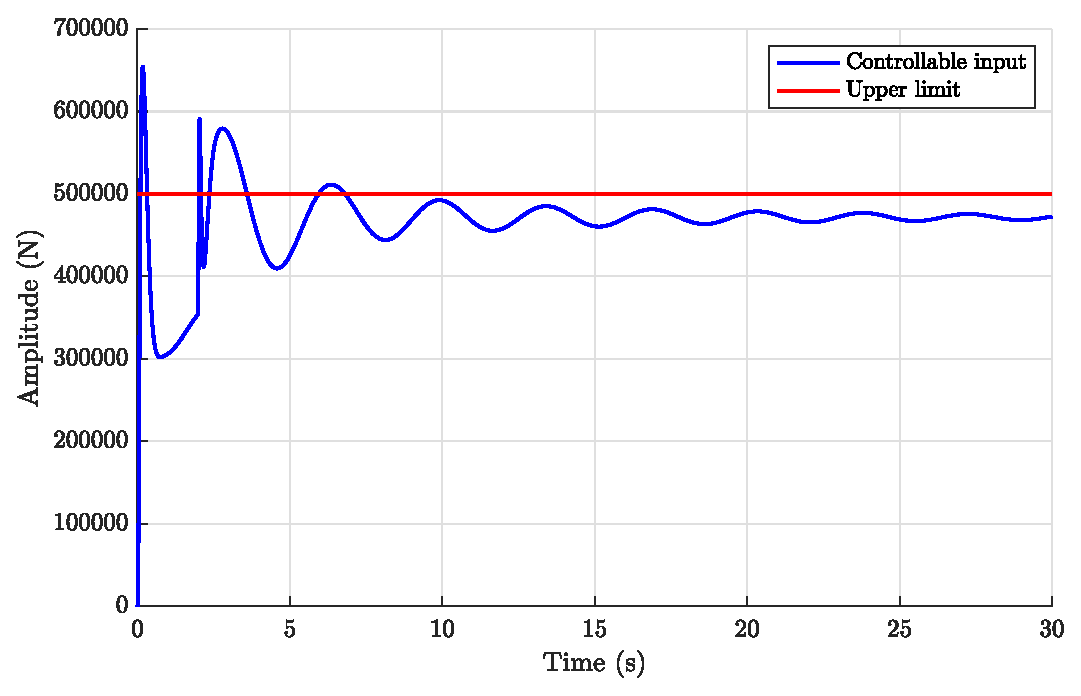
\includegraphics[width=\textwidth]{resources/eps/3_controllable-input.eps}
    \caption{Control input $u(t)$ for $\zeta = \num{0.8}$ and $\omega_c = \num{10}$}
\end{figure}
An abnormally high peak is observed at the beginning. This peak is due to the unrealistic simulations performed : the simulation goes from a zero wind to a constant wind of several thousand newtons in an instant (similar to a step). However, it can be seen that after this peak, the control force oscillates around much more realistic values within our previously defined acceptable range of values.\par
This control input does allow a reduction in building oscillations, and this in a relatively slower way (the system has been slowed down).
\begin{figure}[H]
    \centering
    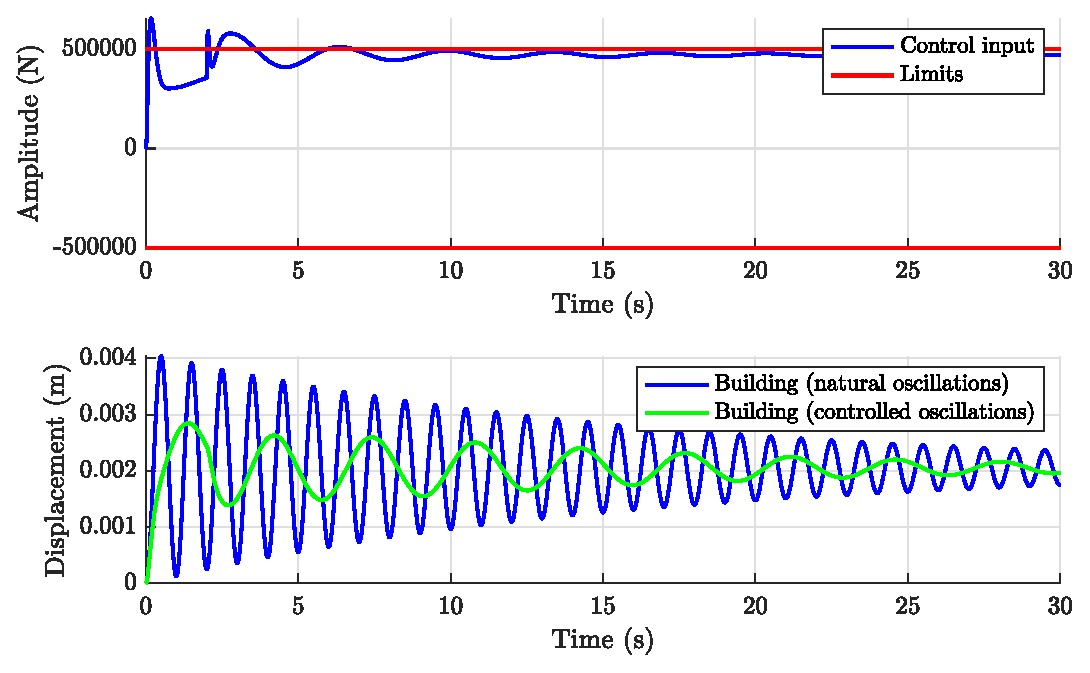
\includegraphics[width=\textwidth]{resources/eps/3_constant.eps}
    \caption{System simulation with and without control input for a constant wind.}
    \label{fig:3.controller}
\end{figure}
We can now evaluate the performance of our observer. To do this, we launched a 10-second simulation with a sinusoidal wind force. In order to observe its convergence, the controlled system and observer have different initial conditions and a time delay upon entry (\SI{2}{\second}).
\begin{figure}[H]
    \centering
    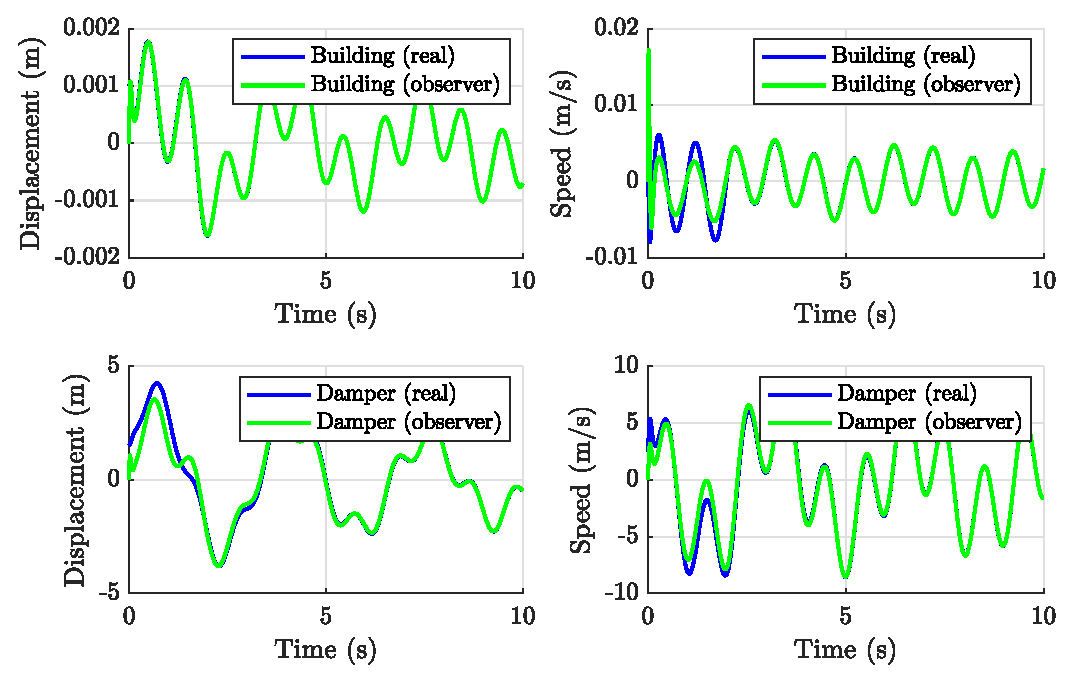
\includegraphics[width=\textwidth]{resources/eps/3_observer.eps}
    \caption{Simulation of the observer with a sinusoidal wind force}
\end{figure}
We notice that our observer converges very quickly (5 seconds maximum, 10 for absolute convergence) towards the real states of the system. Its realization seems to be correct.\par
We can also see that the values of our states, with the control system in place, seem to be consistent and within the plausible value domains we defined earlier.\par
We will now study the behaviour of the system in several situations. We have not plotted the influence of $\zeta$ and $\omega$ as they have an almost identical behaviour as for the previous discussions that led to their determination.

\subsubsection{Response to a reference variation}
For this simulation, we have set the uncontrollable input to 0 and changed the reference to \SI{0.002}{\meter}.
\begin{figure}[H]
    \centering
    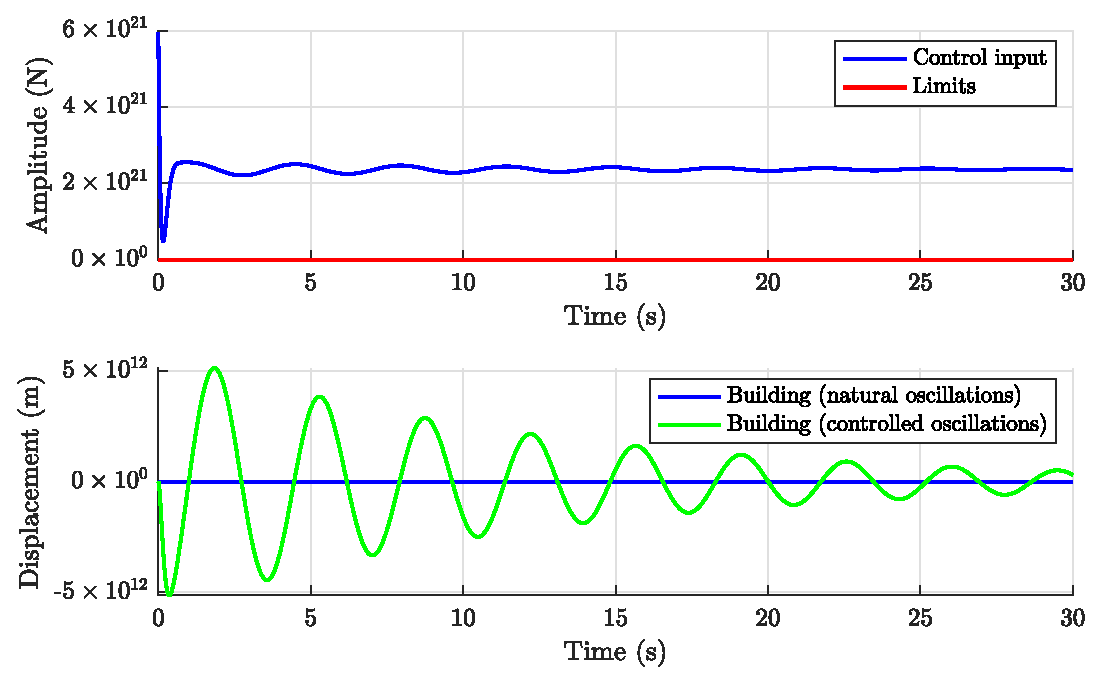
\includegraphics[width=\textwidth]{resources/eps/3_reference.eps}
    \caption{System simulation with a reference variation of \SI{0.002}{\meter}}
\end{figure}
We observe that the values of the controlled signal are totally incoherent. We have not found where this problem comes from. We have designed $k_r$ so that the system is robust to reference variations. The expected behaviour is therefore not normal nor intended.\par
However, the reference of our building is not supposed to change over time, and being resistant to that kind of change is not something we think is needed for this instance.

\subsubsection{Response to a perturbation (disturbance)}
We simulated our different wind scenarios to see how the controlled system reacts. The constant wind scenario has already been presented in figure \ref{fig:3.controller}. We therefore simulated the two remaining scenarios.
\begin{figure}[H]
    \centering
    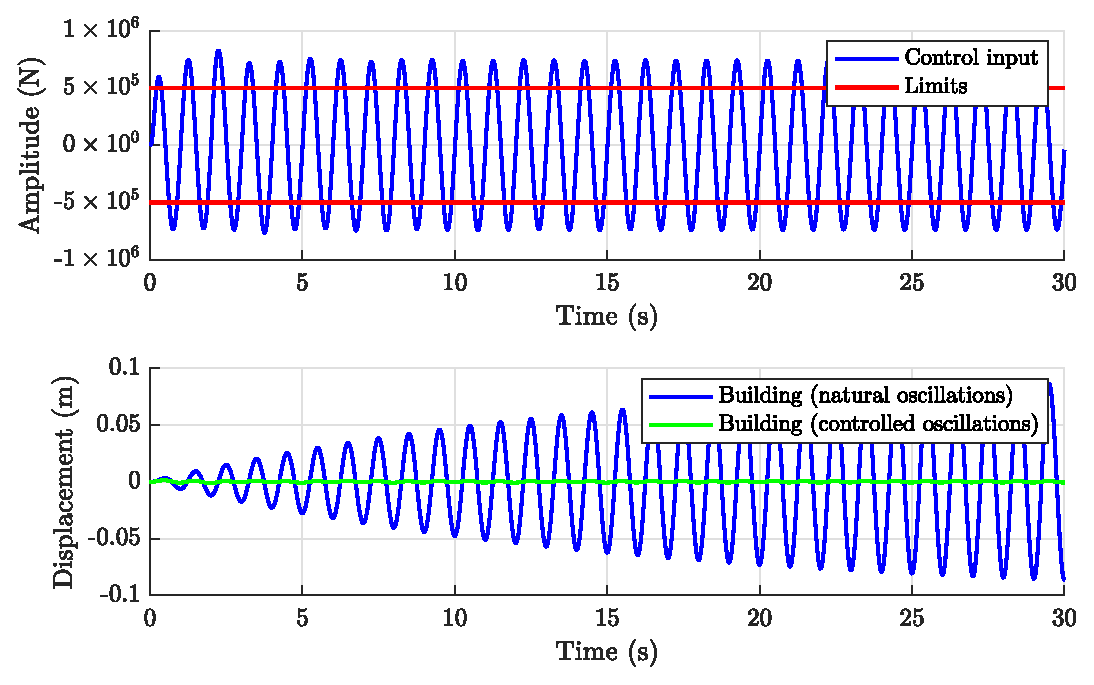
\includegraphics[width=\textwidth]{resources/eps/3_sinusoidal.eps}
    \caption{System simulation with a sinusoidal wind force}
\end{figure}
\begin{figure}[H]
    \centering
    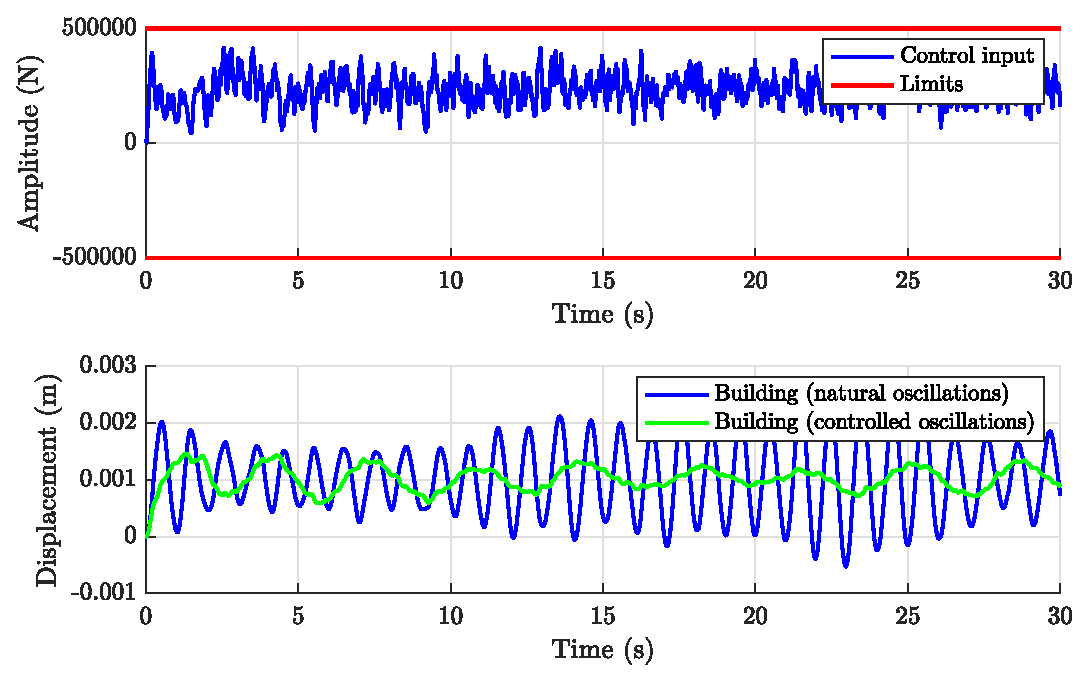
\includegraphics[width=\textwidth]{resources/eps/3_random.eps}
    \caption{System simulation with a random wind force}
\end{figure}
For each of the scenarios, we can see that the oscillations of the buildings are attenuated and tend to disappear completely quite quickly. The controlled system is much slower than the initial system.\par
Our control therefore seems to be fulfilling its role well, although the force we need to apply to our controller is sometimes a bit too high compared to our constraints. We have spent hours trying to reach these constraints by tweaking the parameters of our controller, but this is the best we could manage. More information on that is given in the general conclusion.

\subsubsection{Presence of noise}
For this simulation, we added a random noise (approximately 5\% of the nominal value) to the inputs of the observer (so the output of the controller and the delayed disturbance of the observer). This noise will influence the control input, and therefore the system output.\par
The control input affected by noise is shown in figure \ref{fig:3.noise.control.input}.
\begin{figure}[H]
    \centering
    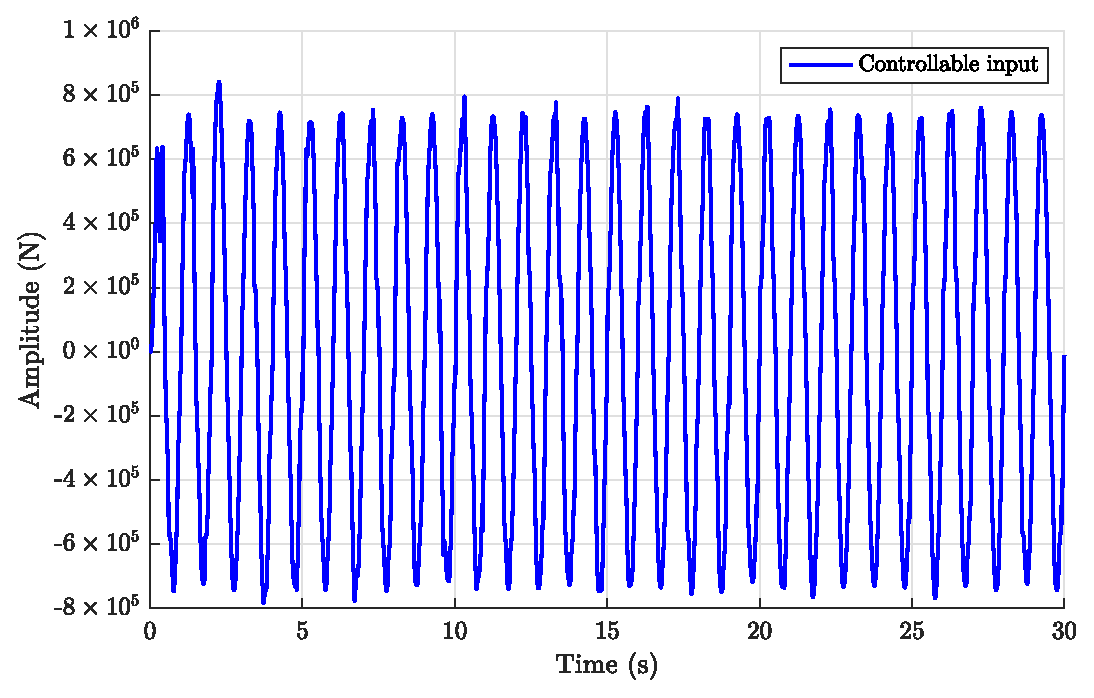
\includegraphics[width=\textwidth]{resources/eps/3_noise-controllable-input.eps}
    \caption{Control input $u(t)$ with noise in the observer}
    \label{fig:3.noise.control.input}
\end{figure}
The system output (as well as the original disturbance) is shown in figure \ref{fig:3.noise}.
\begin{figure}[H]
    \centering
    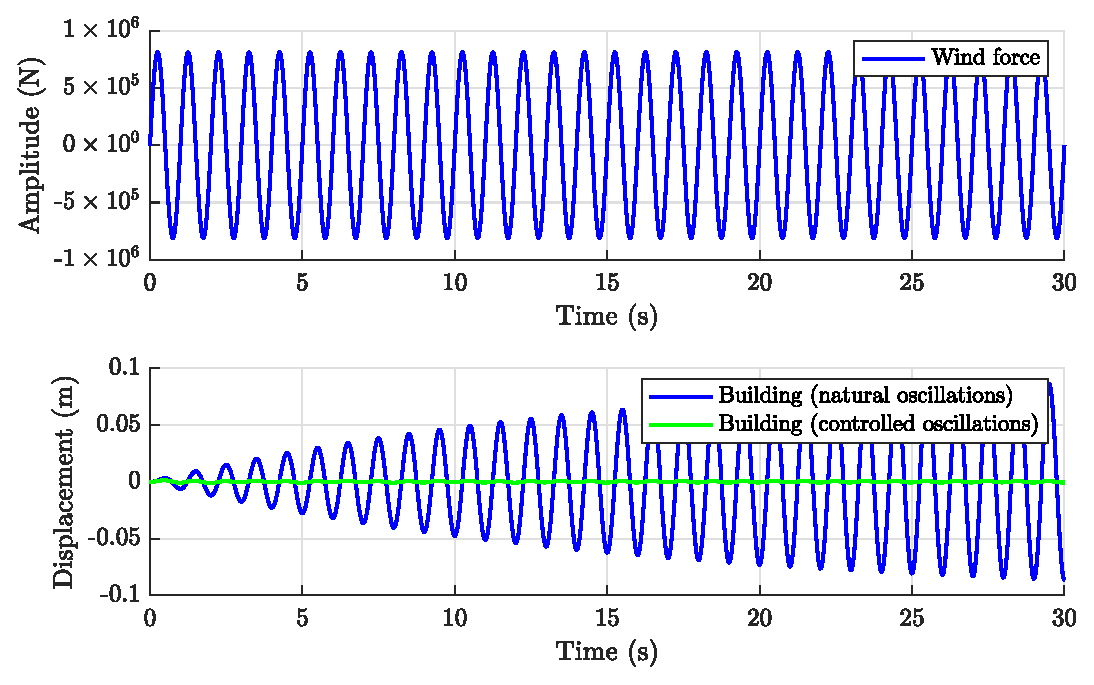
\includegraphics[width=\textwidth]{resources/eps/3_noise.eps}
    \caption{System simulation with noise in the observer}
    \label{fig:3.noise}
\end{figure}
We see that our system is robust to noise. Indeed, despite the presence of the latter, the building's oscillations are still very well attenuated. A try for an explanation is given in the general comparison between the two controllers.
